\section{Architecture}

The final architecture of our project is similar to the one we presented in our midterm project. As the specification requires, the \texttt{gossip} module runs as two independent protocols: one API protocol and one P2P protocol. These two protocols share some data to fulfill the functionality of the module.

\begin{figure}[H]
    \centering
    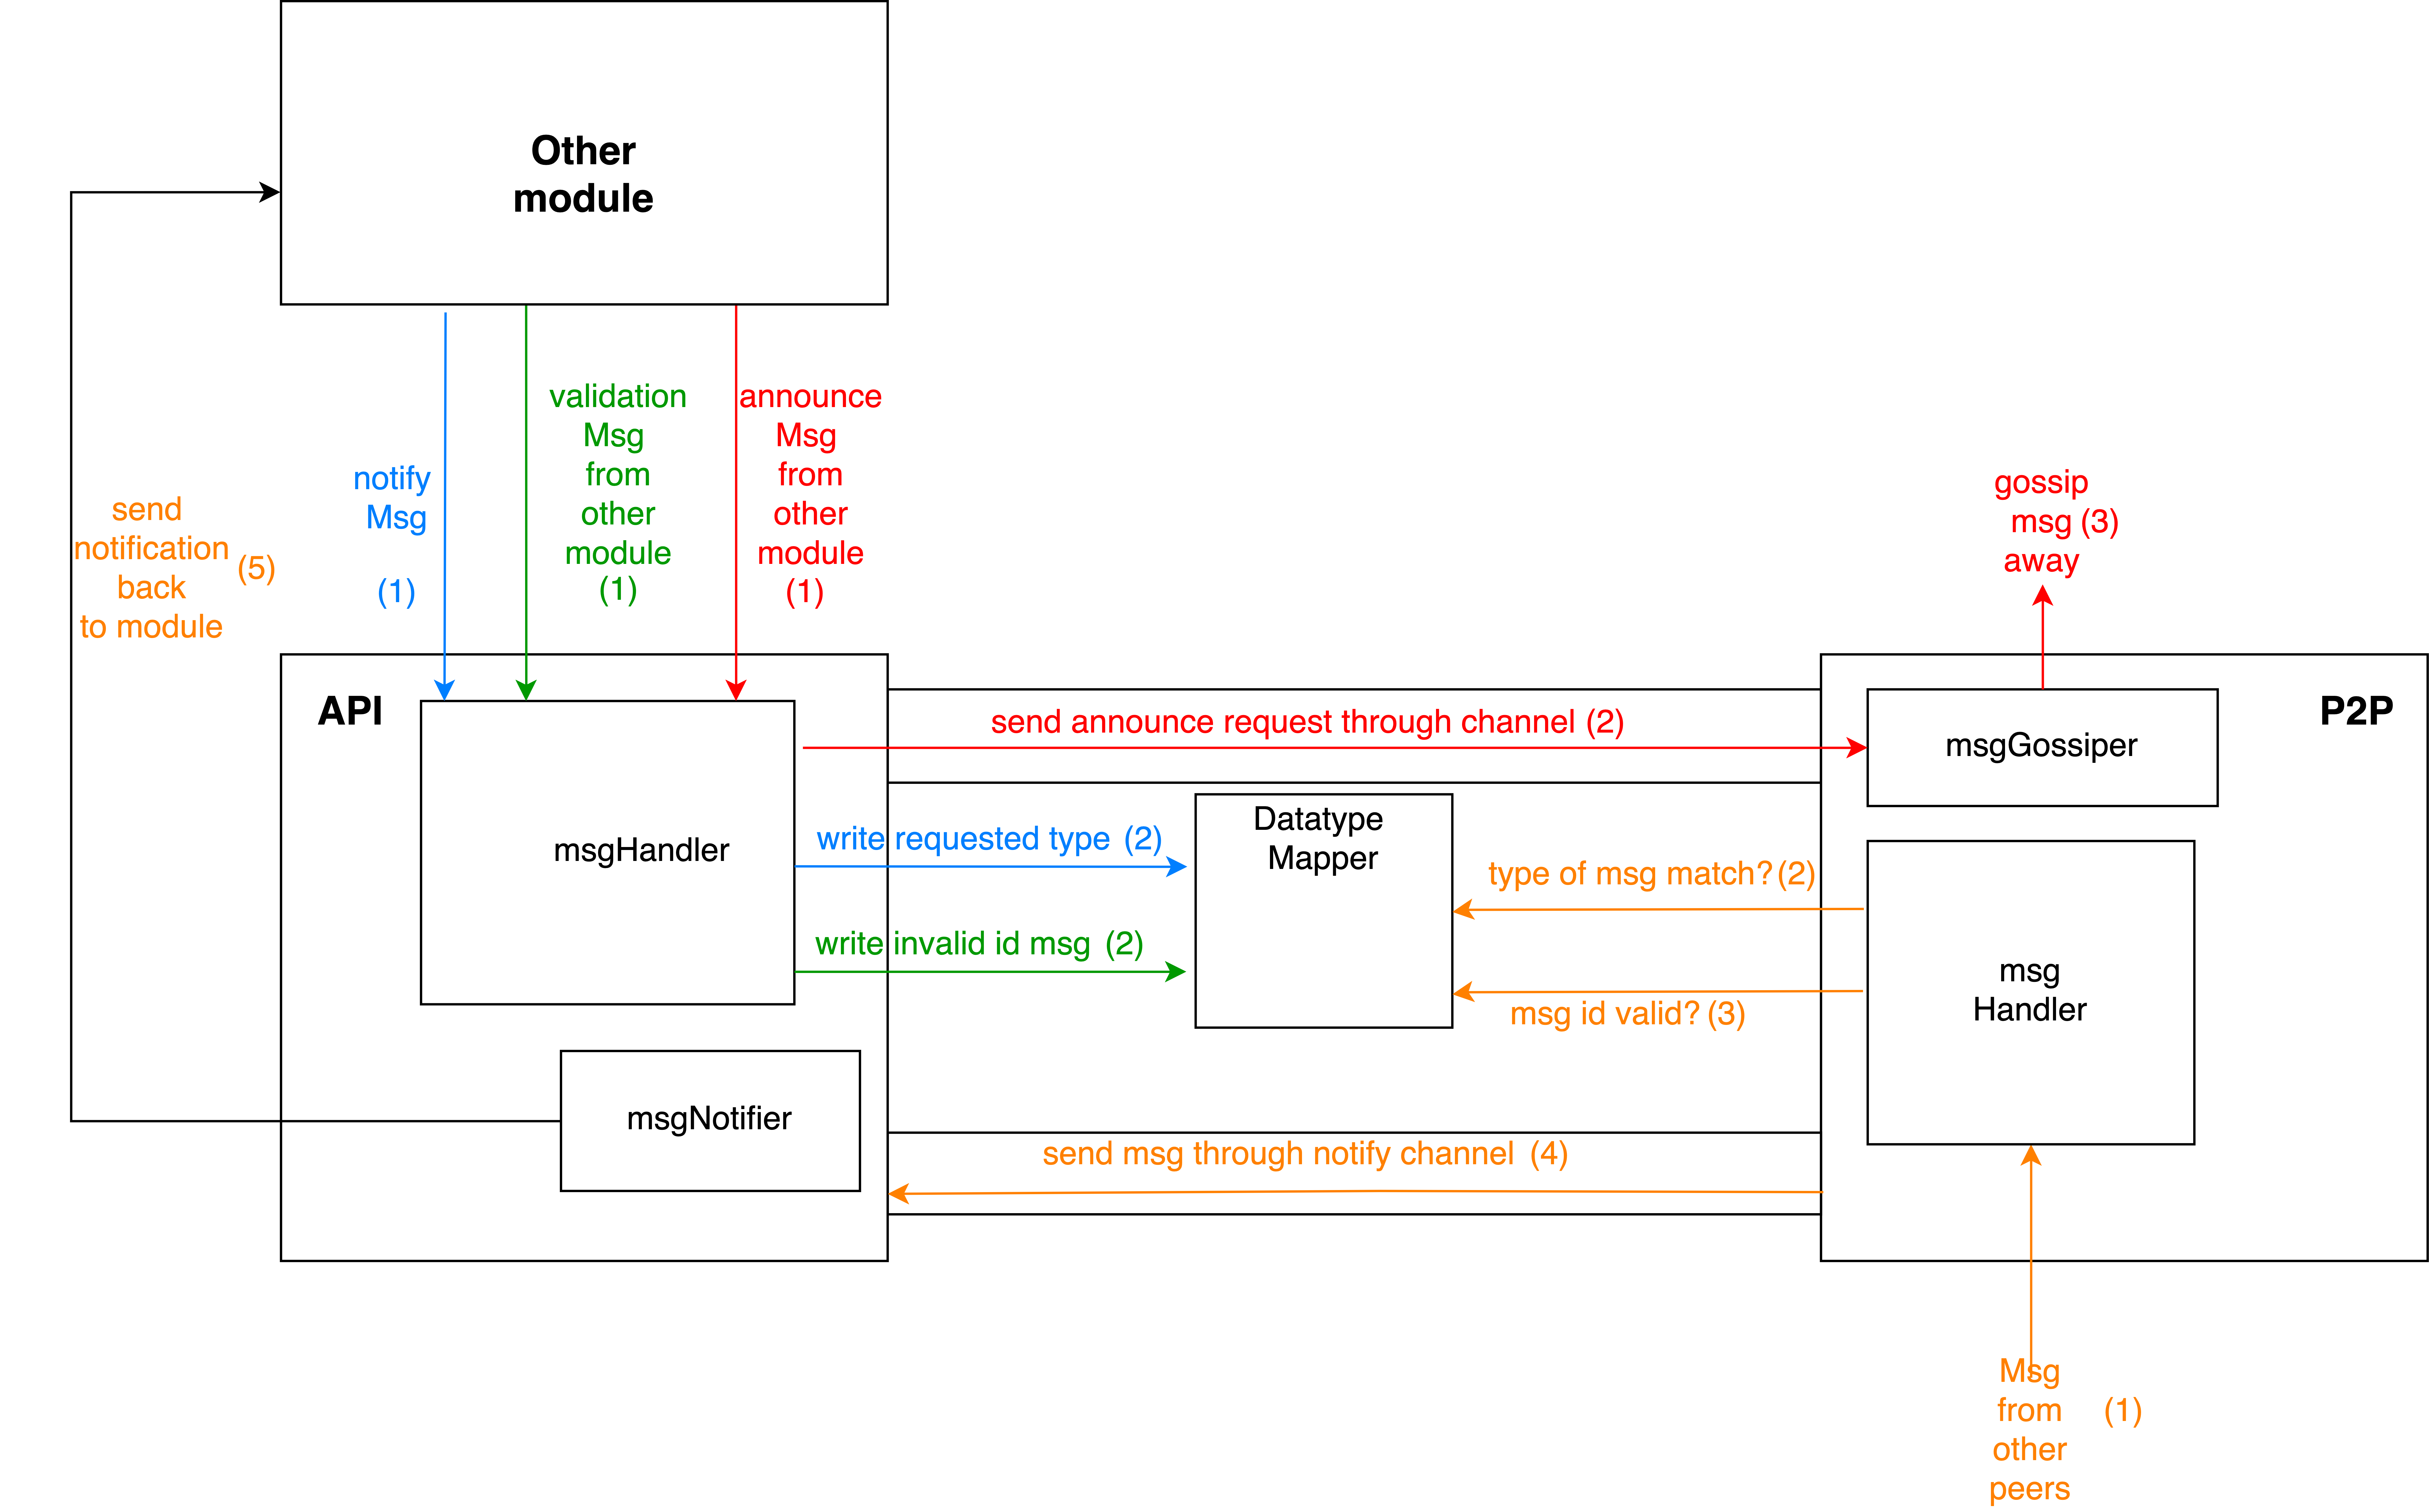
\includegraphics[width=0.85\textwidth]{pics/architecture.png}
    \caption{Structure of the gossip module}
    \label{fig:architecture}
\end{figure}

\subsection{Shared data between API and P2P}

\subsubsection{AnnounceMsgChan}

We have an announce \texttt{Go channel}~\parencite{goChannel} (marked in red in Figure \ref{fig:architecture}) shared between the two protocols. Whenever the \texttt{API} protocol receives an announce message from another module, it processes the message immediately and sends it to the \texttt{P2P} protocol through this channel. The \texttt{P2P} protocol has an announce message handler running on a goroutine that always listens to this channel. When it receives an announce request, it will gossip this message away. 

\subsubsection{DatatypeMapper}

We also need a \texttt{DatatypeMapper} (marked in black in Figure \ref{fig:architecture}) shared between two protocols. Whenever API receives a notify message, it will write the message type that is valid into the mapper and hence should be propagated further. \texttt{DatatypeMapper} also contain a list of invalid message id, which is sent by other module through \texttt{Validation} endpoint. This list is being used by \texttt{P2P} to check for the validity of a message before forwarding it through \texttt{NotiyiMsgChan} 

This datatype mapper will, of course, own a mutex that guarantees no race condition between the two protocols.

\subsubsection{NotiyiMsgChan}

Thanks to the \texttt{DatatypeMapper}, the \texttt{P2P} protocol can recognize which kind of message it should propagate. When it receives a new message, it will check if this message type was requested by any module by reading the datatype mapper and if the message is valid. If that is the case, it sends this message through \texttt{NotiyiMsgChan} (marked in orange in Figure \ref{fig:architecture}). \texttt{API} protocol also has a running goroutine that constantly listens to this channel. It can get those messages from P2P and send corresponding notification messages to the module requesting them. 

\subsection{Security}

We changed our security mechanism according to our midterm feedback. We integrated \texttt{POW} in every gossip message. The hardness of this challenge is defined in the config file. Depending on the security requirement of the project, we can adjust the hardness, also known as the number of leading zeros, accordingly. 

\section{Software Documentation}
\subsection{Important Components and configurations}

\begin{itemize}
    \item \textbf{Node}: The core component responsible for the peer's logic and communication. The node handles traffic from other peers (internode communication) and interactions within the same peer (intranode communication) across the API and P2P modules. It can be customized using the \texttt{config.ini} file to control behavior and parameters.

    \item \textbf{Bootstrapping Service}: A central server responsible for providing initial knowledge to newly joined peers. This service distributes a partial view of the network and designates a set of trusted \texttt{SeedNodes}. The number of \texttt{SeedNodes} can be configured via the \texttt{enum/bootstrapper\_config.go} file, ensuring flexible network deployment.
\end{itemize}


\subsection{How to configure and boot up more nodes}
By default, we have set up the \texttt{docker-compose.yml} file to boot up the bootstrapping service along with three independent nodes. Below is an example of the \texttt{docker-compose.yml} file configuration.

For more details, take a look at the \texttt{docker-compose.yml}

 \textbf{Ports:} For each node, we map local ports to container ports. For example:
  \begin{itemize}
    \item \texttt{"9002:9000"} maps traffic from \texttt{localhost:9002} to \texttt{node:9000}.
    \item \texttt{"9003:9001"} maps traffic from \texttt{localhost:9003} to \texttt{node:9001}.
  \end{itemize}
It's crucial to set these ports correctly to enable the client code to interact with the respective nodes.

 \textbf{Container Names:} Each container has a unique name, such as \texttt{node}, \texttt{node1}, and \texttt{node2}, ensuring no conflicts.

\textbf{Networks:} All containers must be in the same network (e.g., \texttt{my-network}) to correctly enable communication.

\textbf{Volumes:} Each node's configuration is mounted from the \texttt{docker-container-config} folder to the container, e.g., \texttt{./docker-container-config/config-node:/root/configs}. Ensure you provide the correct path to the configuration file.

Additionally, the \texttt{config.ini} file for each node should have a unique \texttt{p2p\_address} to prevent conflicts, as shown in the sample \texttt{config.ini}:

\begin{figure}[H]
    \centering
    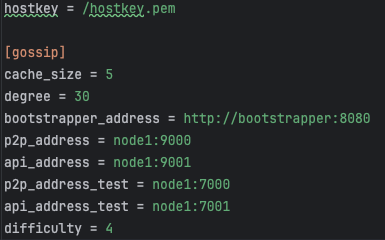
\includegraphics[width=0.75\textwidth]{pics/config.png}
    \caption{Sample configuration file}
    \label{fig:config}
\end{figure}

For example: \texttt{node1:9000} and \texttt{node1:9001} for \texttt{node1}. And \texttt{node2:9000} and \texttt{node2:9001} for \texttt{node2}.

\subsubsection{Boot up more nodes:}
  \begin{itemize}
    \item \textbf{Step 1:} add new config.ini file to \texttt{./docker-container-config} Make sure config.ini resides in a uniquely named folder according to the node you want to inject the config.int to. For example: \texttt{node10-config} should be injected into \texttt{node10}
    \item \textbf{Step 2:} adjust \texttt{docker-compose.yml} accordingly. Add new entry to \texttt{services:} section. Make sure the path to config.ini is set correctly.
  \end{itemize}
  
  
\subsection{Additional Logic To P2P Protocol}

\subsubsection{Peer Join:}
When a peer joins the network, it needs to notify other peers to become part of the distributed system. This is done by sending a \texttt{PeerJoinAnnounce} message to all known peers. The joining peer sends out its address, which is then propagated through the network using the gossip protocol. This ensures all active peers update their local peer list with the new node.

Key steps:
\begin{itemize}
    \item The new peer sends a \texttt{PeerJoinAnnounce} message.
    \item Existing peers receive this message and add the new peer to their local list.
    \item The message propagates via the gossip protocol to ensure network-wide awareness.
\end{itemize}

\subsubsection{Peer Leave:}
When a peer leaves the network, it announces its departure by sending a \texttt{PeerLeaveAnnounce} message. This ensures the departing peer is removed from the other peers' lists. The peer sends this message to its known peers, who propagate the information using gossip to ensure all peers update their lists.

Key steps:
\begin{itemize}
    \item The leaving peer sends a \texttt{PeerLeaveAnnounce} message.
    \item Existing peers remove the peer from their local peer lists.
    \item The message is gossiped across the network, updating all peers.
\end{itemize}

\subsubsection{Request Peer List:}
A peer can request the peer list from another node to maintain an up-to-date view of the network. The requesting peer sends a \texttt{PeerListRequest} message, prompting the target peer to respond with its list of known peers. This ensures nodes remain aware of each other, particularly after membership changes.

Key steps:
\begin{itemize}
    \item The requesting peer sends a \texttt{PeerListRequest} message.
    \item The target peer responds with its current list of peers.
\end{itemize}

\subsubsection{Response Peer List:}
When receiving a \texttt{PeerListRequest}, the peer responds with a \texttt{PeerListResponse} message, containing its current list of known peers. This allows the requesting peer to update its peer list accordingly and keeps the network synchronized.

Key steps:
\begin{itemize}
    \item The peer receiving the request sends a \texttt{PeerListResponse} with its peer list.
    \item The requesting peer updates its list based on the response.
\end{itemize}



\section{How to install and run}
To install and run the project, follow the steps below:

\begin{enumerate}
    \item \texttt{git clone} the project repository to your local machine:
    \begin{verbatim}
    git clone <repository-url>
    \end{verbatim}

    \item Install \texttt{Docker Engine} on your system if it is not already installed. Please follow the instructions on \href{https://docs.docker.com/}{Docker's official site.}

    \item Make the build script executable by running (make sure you are in the project directory):
    \begin{verbatim}
    chmod +x build.sh
    \end{verbatim}

    \item Run the build script that includes all necessary commands to pull build docker images and run them up:
    \begin{verbatim}
    ./build.sh
    \end{verbatim}

After the step above, you should be able to observe the behavior of the containers 

The steps underneath are optional if you want to use our Go client. You can also interact with the running Nodes by using the Python client provided in the course.

    \item (Optional) Install \texttt{Go} to ensure the Go environment is properly set up.

    \item (Optional) Run Go Client to interact with node. For more details, take a look at Readme.md.
    \begin{verbatim}

    \end{verbatim}
\end{enumerate}


\subsection{Known Issues}

\begin{itemize}
    \item \textbf{Node Leave}: Currently, the node leave mechanism is not functioning correctly. The node fails to send a gossip message before shutting down completely. The reason may be due to using TCP instead of UDP for sending messages, which leads to delays and failed messages when a peer tries to read PeerLeaveAnnounce from the closed TCP connection.
    
    \item \textbf{Bootstrapping Inefficiencies}: The bootstrapping strategy is not optimized. Peer discovery can be slow and inefficient, especially in larger networks.
    
    \item \textbf{Seed Node Refresh}: There is no mechanism for peers to refresh their view of seed nodes if one of the seed nodes goes offline. This can lead to outdated peer lists and network instability.
    
    \item \textbf{Seed Node Assignment}: Any peer who joins the network first becomes a seed node. If a seed node goes offline, the next joining node becomes a seed node, which can yield issues with network stability.
\end{itemize}

\section{Future Work}

\begin{itemize}
    \item \textbf{Improve Node Leave Mechanism}: Implement a more robust mechanism to handle node departure. Currently, nodes fail to send the gossip message before shutting down completely. Switching from TCP to UDP for leave notifications would allow faster, more reliable communication before the node exits.

    \item \textbf{Optimize Bootstrapping Strategy}: The current bootstrapping strategy has inefficiencies and should be optimized to prevent issues like inconsistent peer discovery and poor handling of network partitioning.

    \item \textbf{Seed Node Refresh Mechanism}: Develop a dynamic seed node refresh mechanism to allow peers to refresh their view of seed nodes. This is especially necessary when one of the seed nodes goes offline, so the network can remain stable without depending on unreachable nodes.

    \item \textbf{Redesign Seed Node Assignment}: The current logic assigns the first peer as a seed node, and if a seed node goes offline, the next joining node becomes a seed node. This can lead to instability. The seed node assignment mechanism should be more robust, ensuring stable and capable nodes are assigned as seed nodes.
    
    \item \textbf{Peer View Synchronization}: Work on synchronizing peer lists more efficiently across nodes, particularly in the event of network partitions or if a large number of nodes join simultaneously.
    
    \item \textbf{Security Enhancements}: Explore more advanced security protocols for P2P communication beyond proof of work, such as mutual authentication or encryption, to enhance the integrity and confidentiality of gossip messages.
\end{itemize}

\section{Workload Distribution}
Our previous distribution of tasks has worked very well, ensuring smooth collaboration and efficient development. The responsibilities were divided as follows:

\begin{itemize}

    \item \textbf{Thua Duc Nguyen}: in charge of implementing the API server, designing the overall architecture of the peer, and developing security measures. Additionally, Duc implemented the Go client to facilitate testing and provided scripts that streamlined Docker container building and execution processes.
    
    \item \textbf{Duc Trung Nguyen}:  responsible for designing and implementing the core P2P protocols, including the bootstrapping mechanism. Additionally, Trung handled dockerizing the application, allowing seamless config file injection into containers and ensuring flexible deployment strategies.

\end{itemize}

This clear division of tasks allowed us to effectively meet our deadlines and achieve the project goals.
